\documentclass[12pt, handout]{beamer}
\geometry{letterpaper,landscape}
\setbeamersize{text margin left=30mm,text margin right=30mm}

\usepackage{graphicx}
\usepackage[utf8]{inputenc}

\usebackgroundtemplate%
{%
	
\includegraphics[width=\paperwidth]{background.png}%
}

\begin{document}
	\begin{frame}{Demonstrations}
		\parbox{\linewidth}
		{
			Nuestro objetivo principal es motivar a los estudiantes sobre el estudio de la computación como herramienta para la exploración de diversidad de problemas junto con su resolución, usando Python como herramienta principal. Esto con el fin que en el futuro puedan desarrollar un razonamiento lógico aplicado a la creación de algoritmos. 
		}
		
		\vspace{0.5cm}
		\parbox{\linewidth}
		{
			Se busca que con esta idea se puedan implementar estos ejemplos como experimentos demostrativos, análogos a los que actualmente se realizan en Física 1 y Física 2.
		}
		
		\vspace{0.25cm}
		\url{https://github.com/ComputoCienciasUniandes/Demonstrations}
		\begin{itemize}
			\begin{columns}[t, onlytextwidth]
				\column{.19\textwidth}
					\item \textbf{Pendulum}
					
					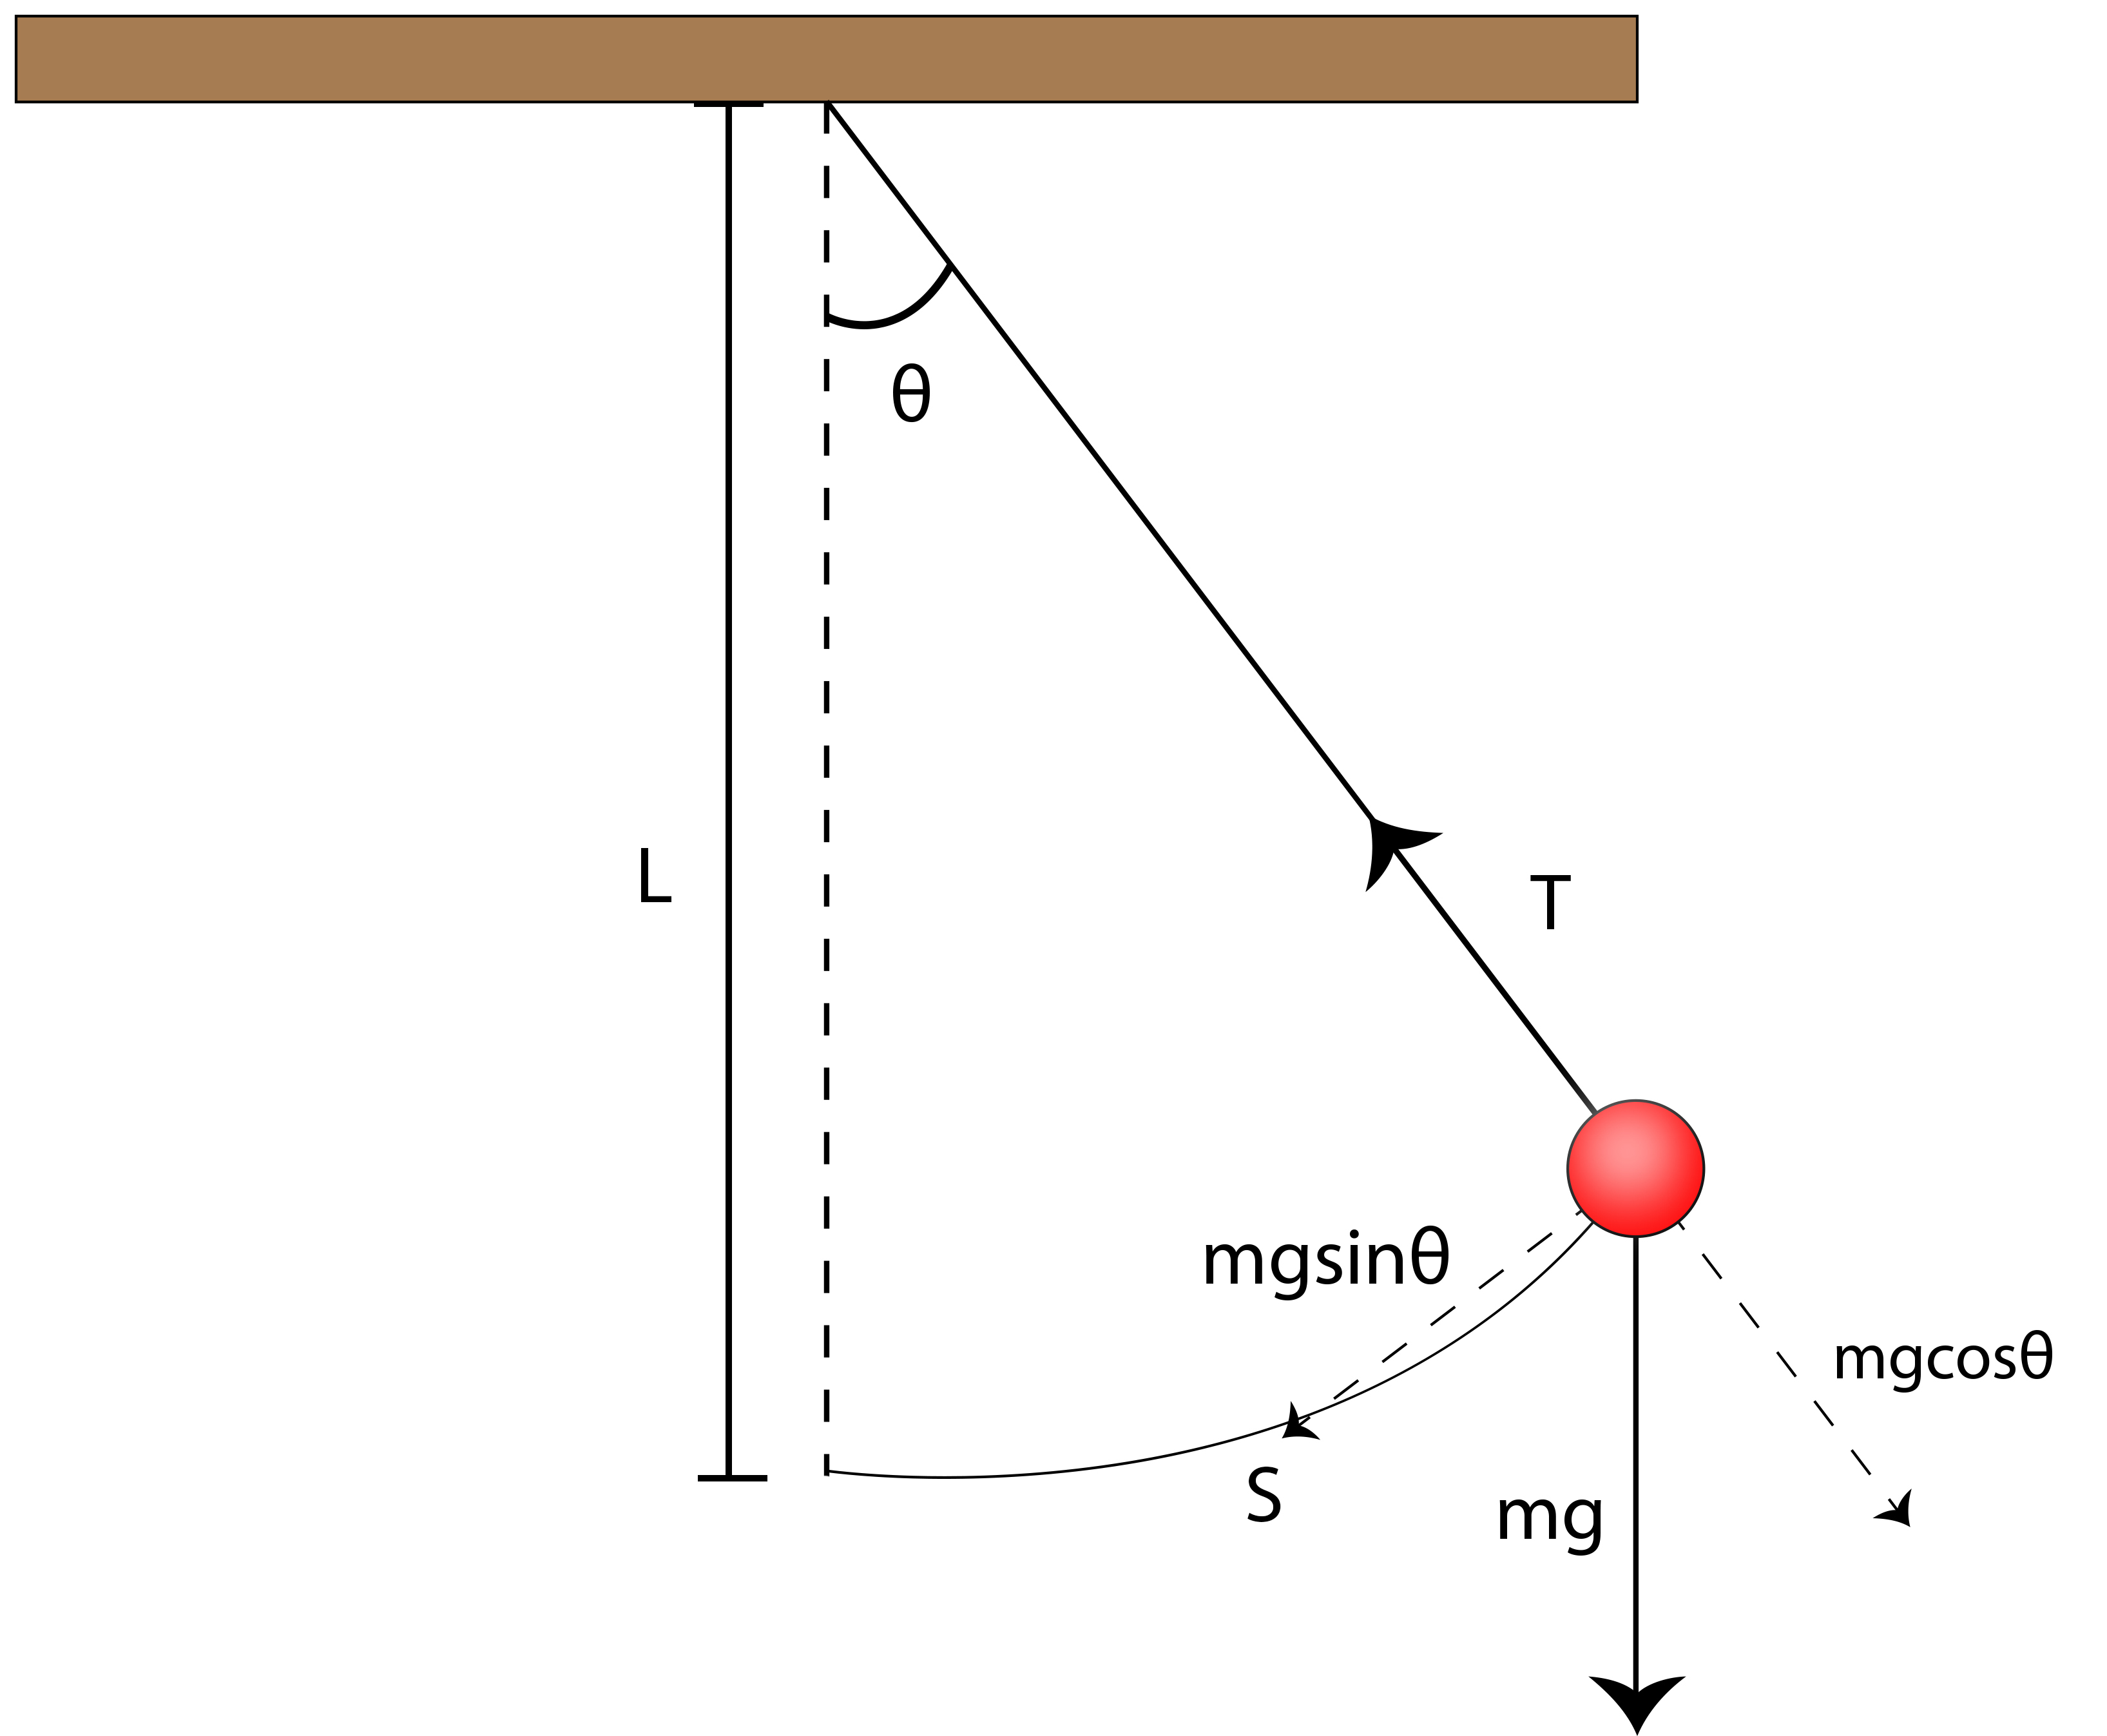
\includegraphics[width = \linewidth]{../Pendulum/Pendulum.jpg}
					\begin{equation*}
						\ddot{\theta} = -\dfrac{g}{L}\sin\theta
					\end{equation*}
				
				\column{.19\textwidth}
					\item \textbf{ProjectileMotion}
					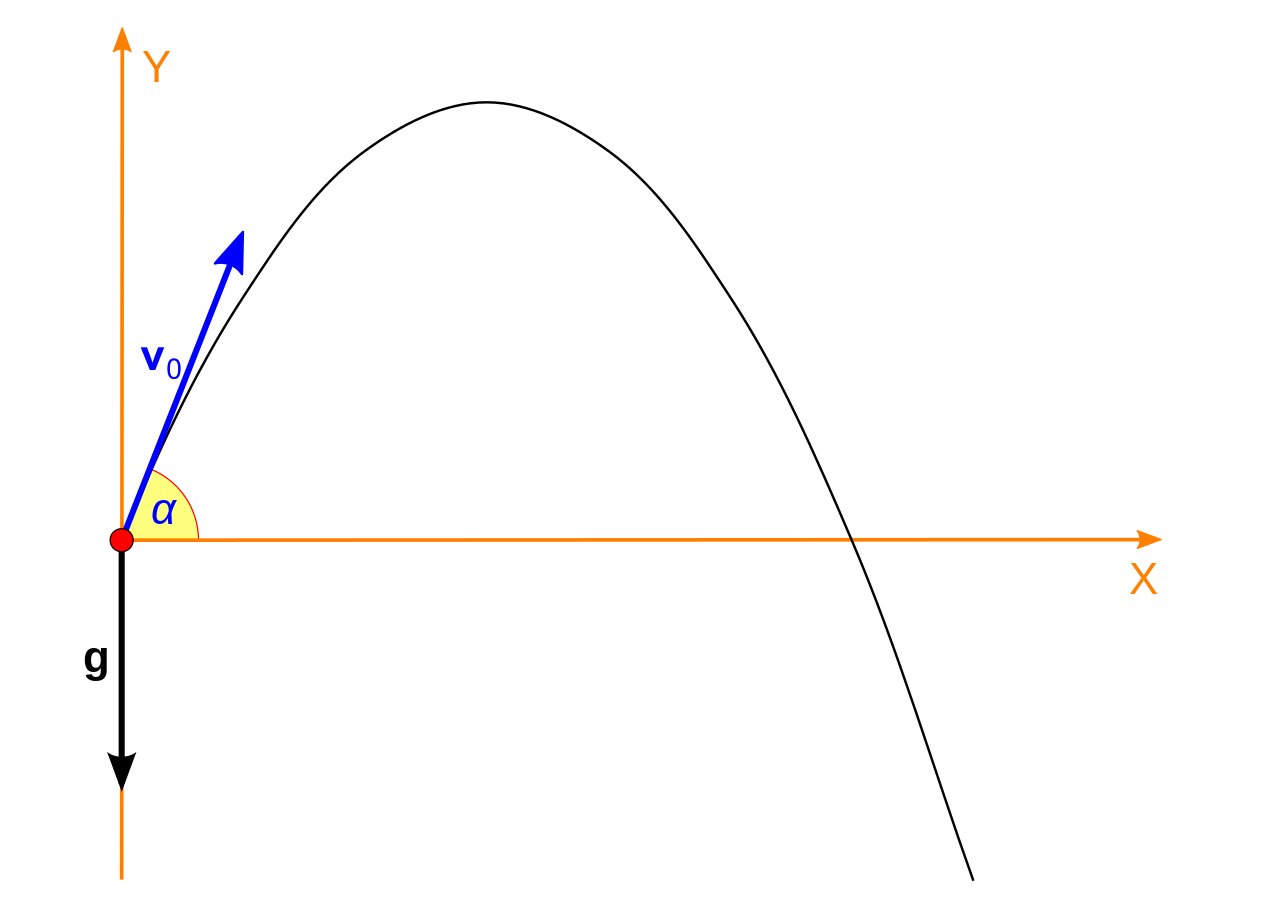
\includegraphics[width = \linewidth]{../ProjectileMotion/projectile.png}
					\begin{equation*}
						\ddot{x} = -\dfrac{\beta}{m}\dot{x}
					\end{equation*}
					\begin{equation*}
						\ddot{y} = -\dfrac{\beta}{m}\dot{y} - mg
					\end{equation*}
				
				\column{.19\textwidth}
					\item \textbf{SolarSystem}
					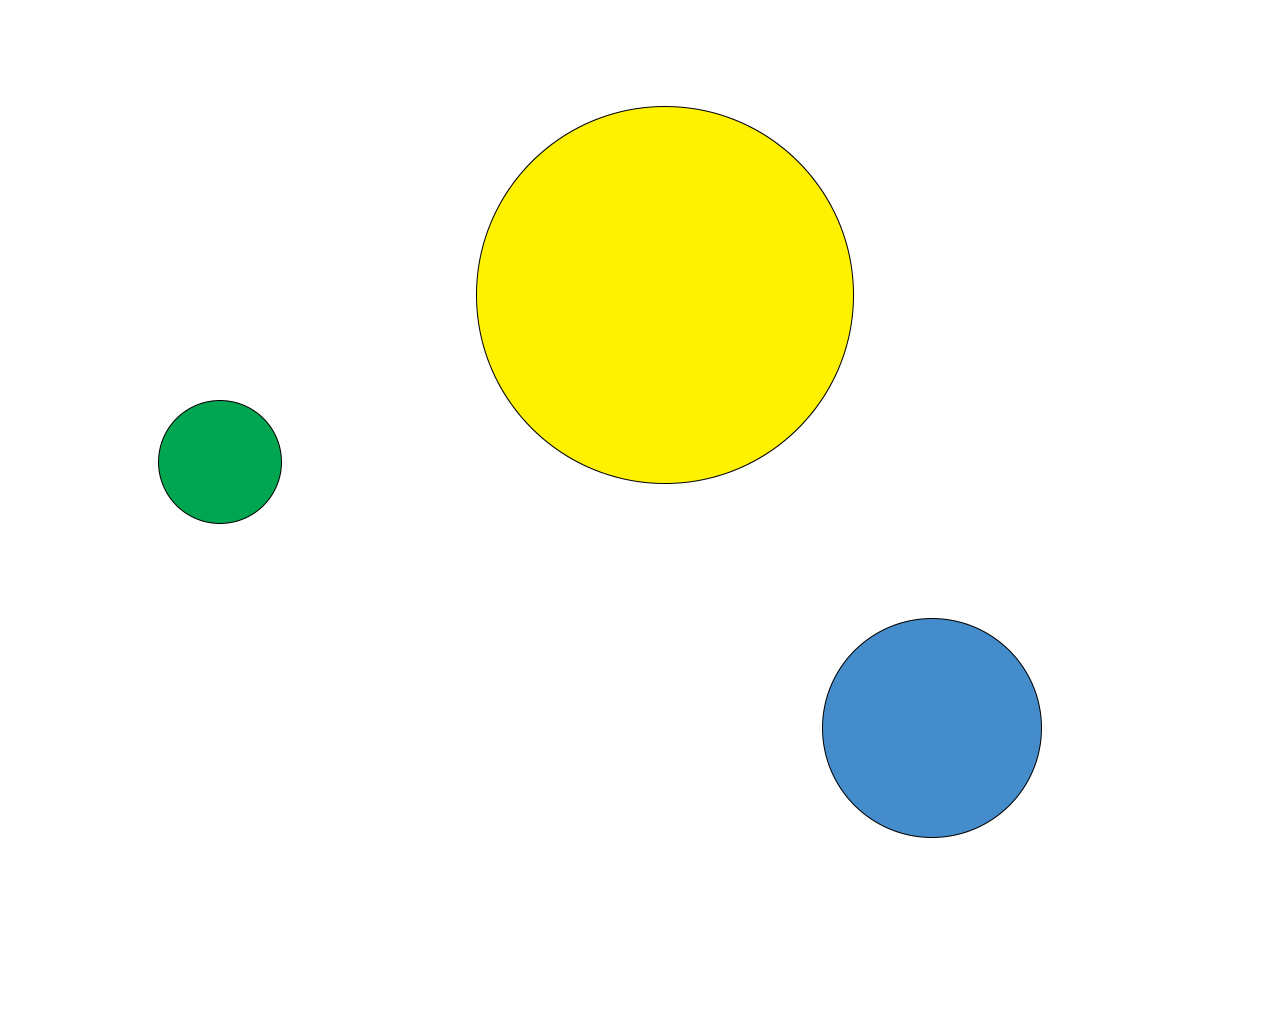
\includegraphics[width = \linewidth]{../SolarSystem/system.jpg}
					\begin{equation*} 			\ddot{\vec{r}}_i= G\sum\limits_{i\neq j}^{N} \frac{m_j}{|\vec{r}_{ij}|^3}(\vec{r}_j - \vec{r}_i)
					\end{equation*}
				
				\column{.19\textwidth}
					\item \textbf{SpringPendulum}
					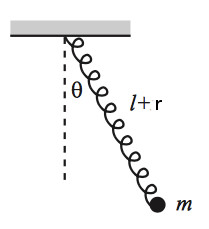
\includegraphics[width = \linewidth]{../SpringPendulum/spring.jpg}
					\footnotesize
					\begin{equation*}
					\ddot{r} = (l+r)\dot{\theta}^2 + g\cos\theta - \omega^2r
					\end{equation*}
					\begin{equation*}
					\ddot{\theta} = -\dfrac{1}{l+r}\left(2\dot{r}\dot{\theta}+g\sin\theta\right)
					\end{equation*}
				
				\column{.19\textwidth}
					\item \textbf{DoublePendulum}
					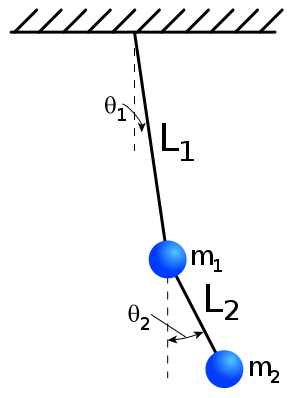
\includegraphics[width = \linewidth]{../DoublePendulum/pendulum.png}
					
			\end{columns}
			\vspace{0.5cm}
			\begin{columns}[t, onlytextwidth]
				\column{.19\textwidth}				
					\item Fuerzas
					\item Condiciones iniciales interactivas
				
				\column{.19\textwidth}			
					\item Fuerzas
					\item Condiciones iniciales interactivas
				
				\column{.19\textwidth}
					\item Fuerzas
					\item Datos reales de NASA Horizon
				
				\column{.19\textwidth}
					\item Energías (Lagrangiano)
				
				\column{.19\textwidth}
					\item Energías (Lagrangiano)
					\item Uso de cálculo simbólico
			\end{columns}
			\vspace{1cm}
			\begin{columns}[t, onlytextwidth]
				\column{.19\textwidth}				
					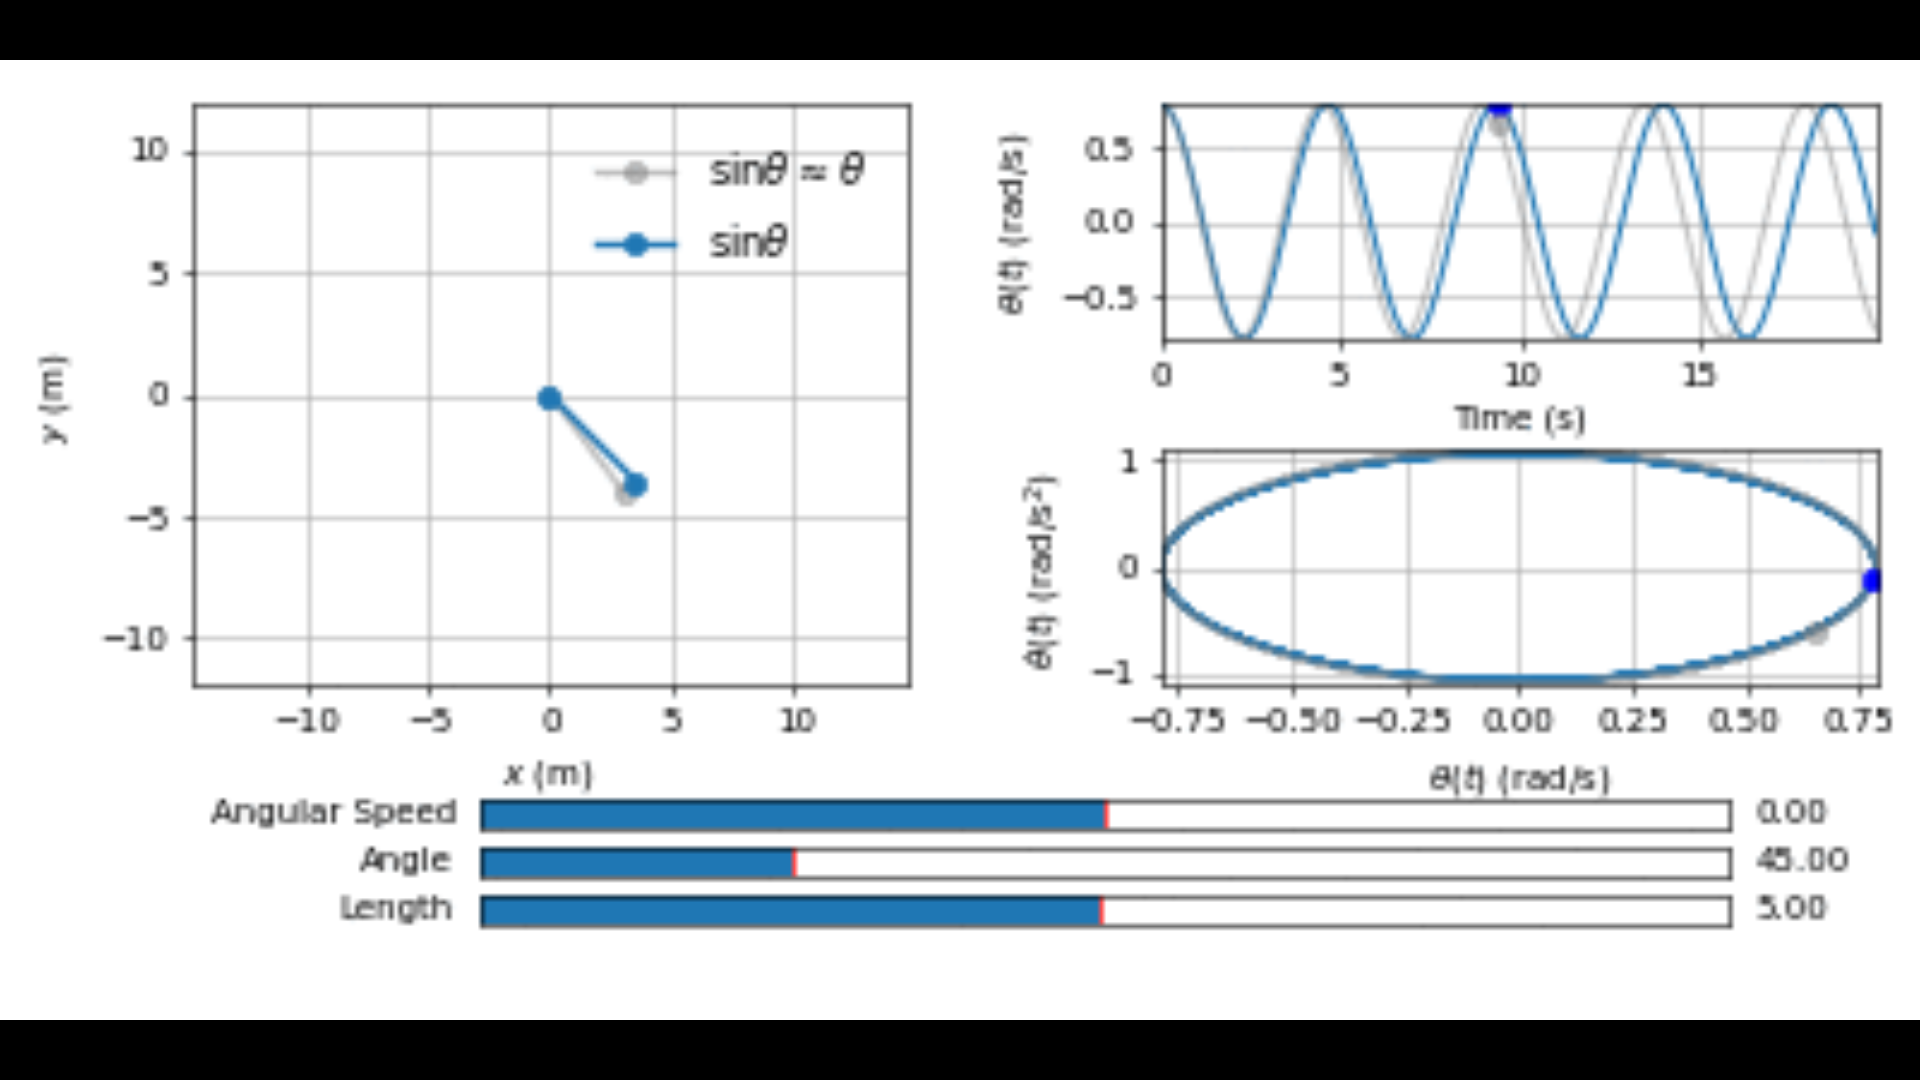
\includegraphics[width = \linewidth]{P.png}
				
				\column{.19\textwidth}			
					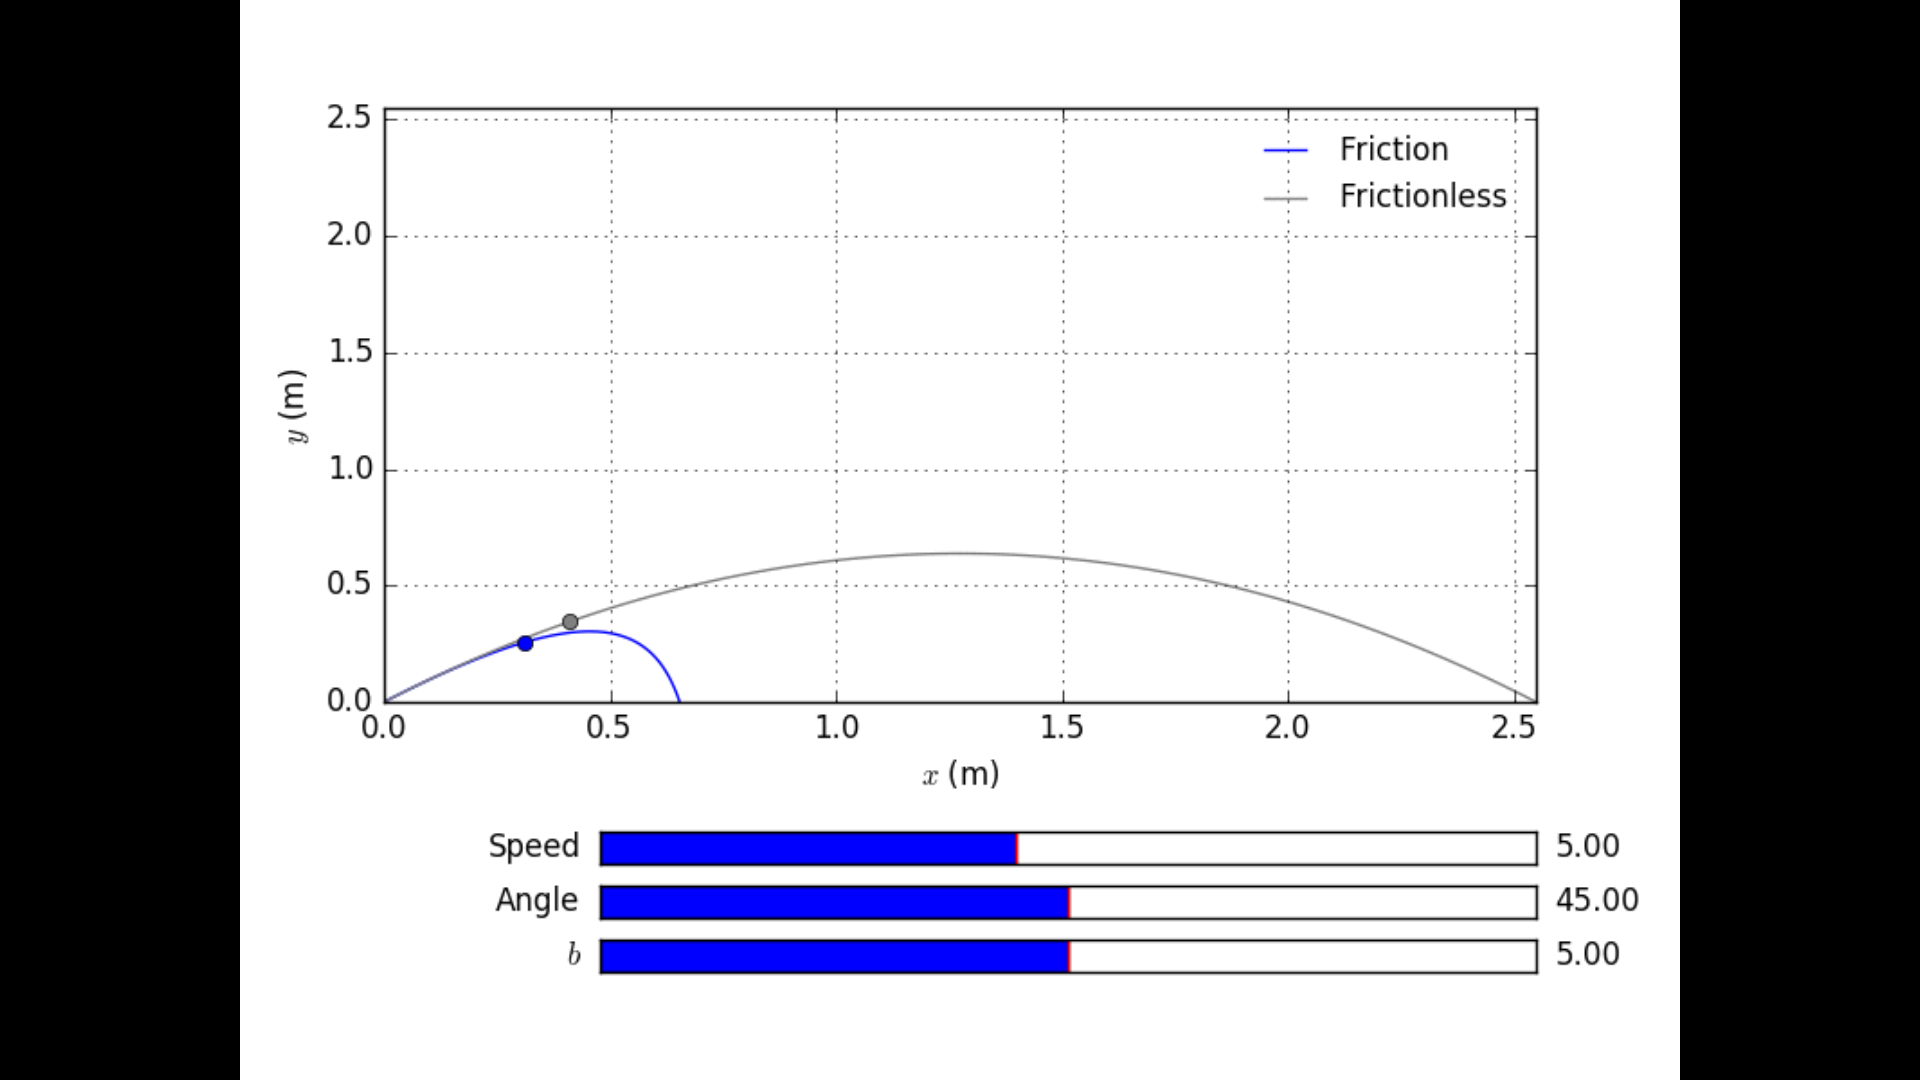
\includegraphics[width = \linewidth]{PM.png}
				
				\column{.19\textwidth}
					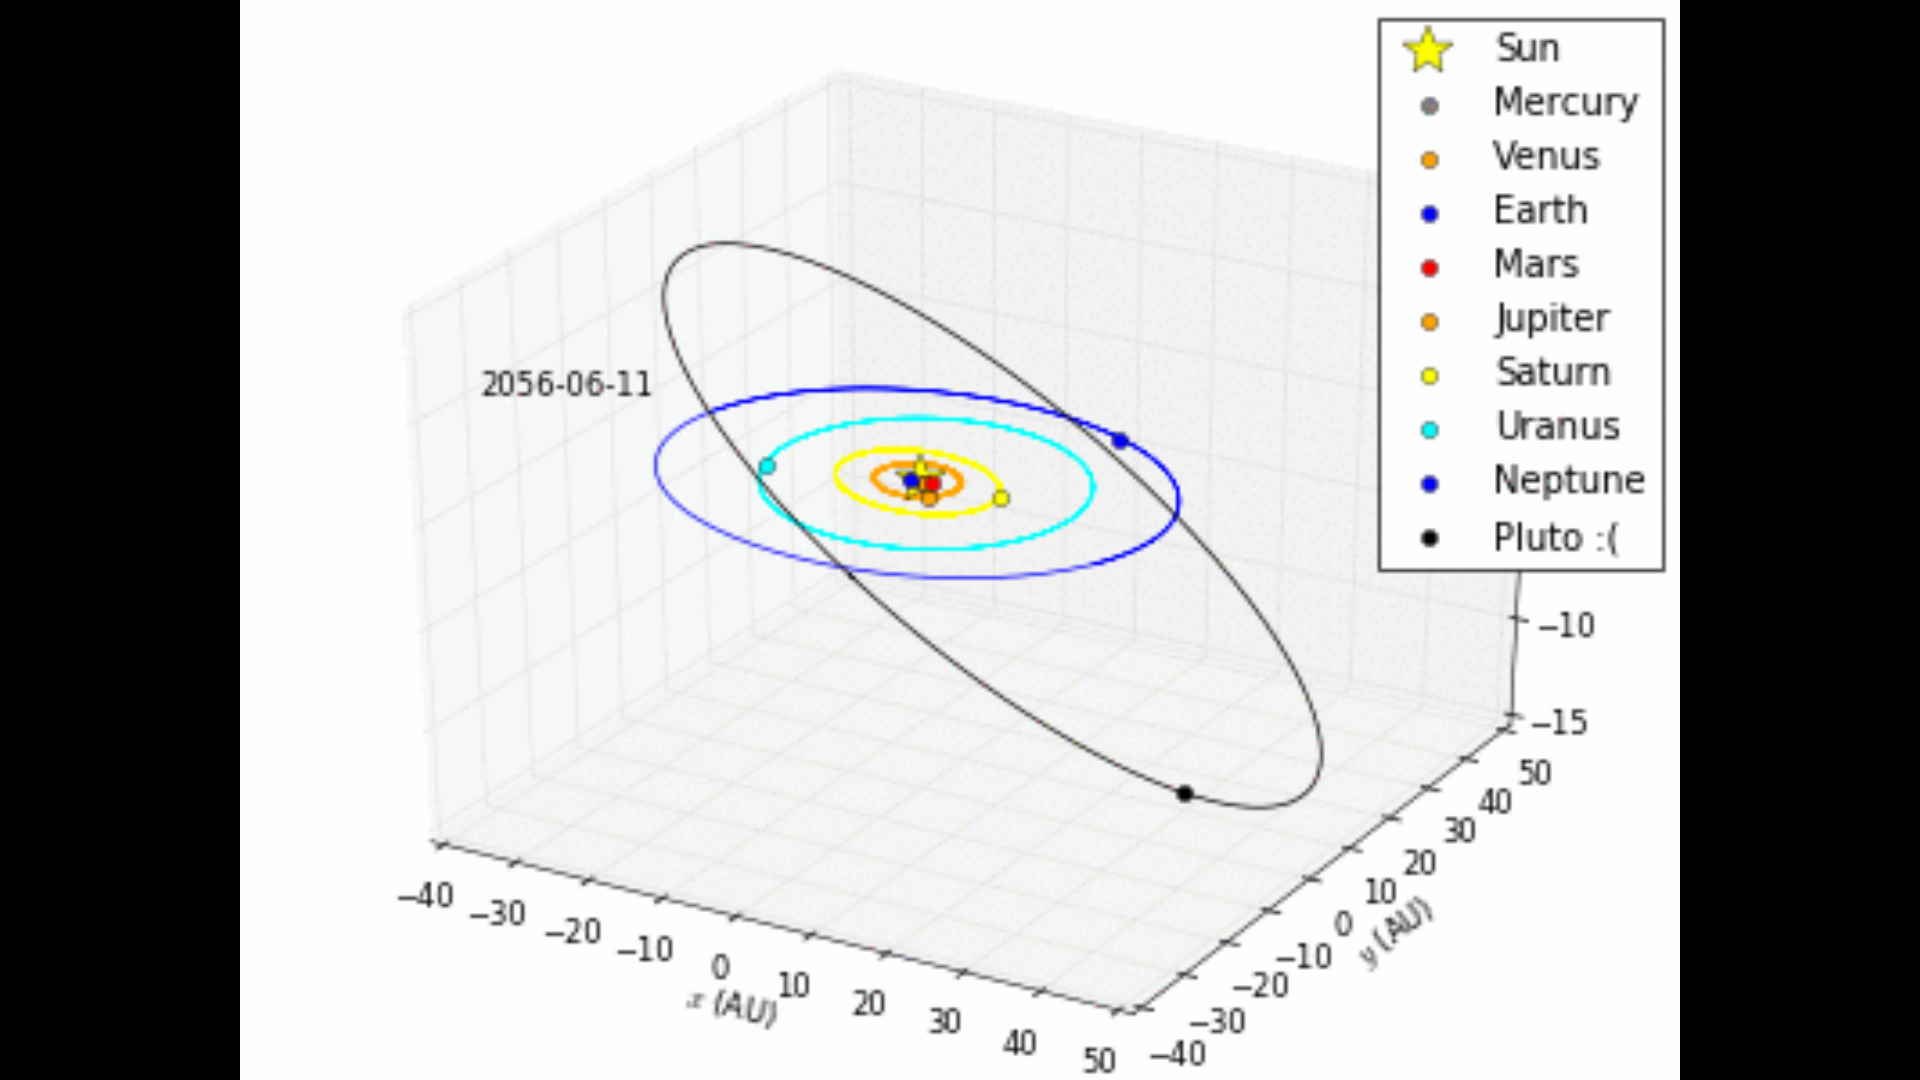
\includegraphics[width = \linewidth]{SS.png}
				
				\column{.19\textwidth}
					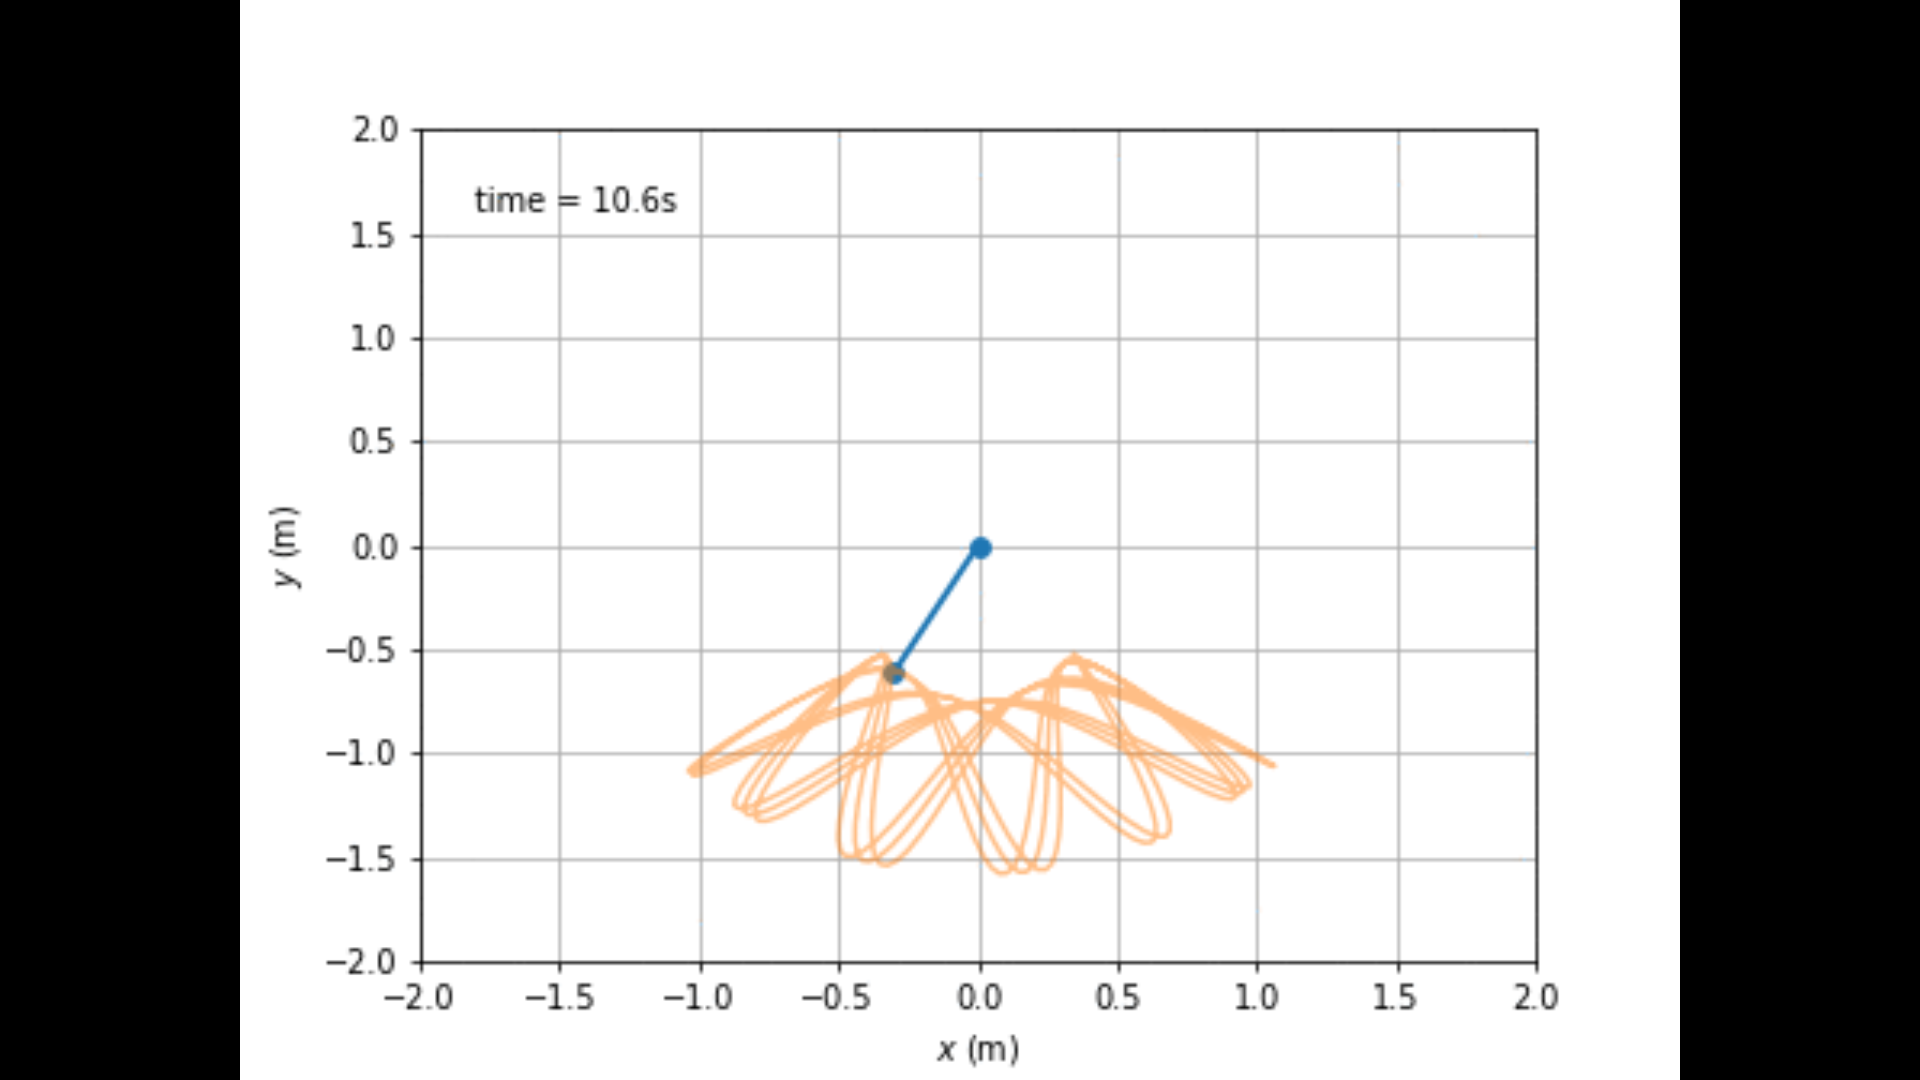
\includegraphics[width = \linewidth]{SP.png}
				
				\column{.19\textwidth}
					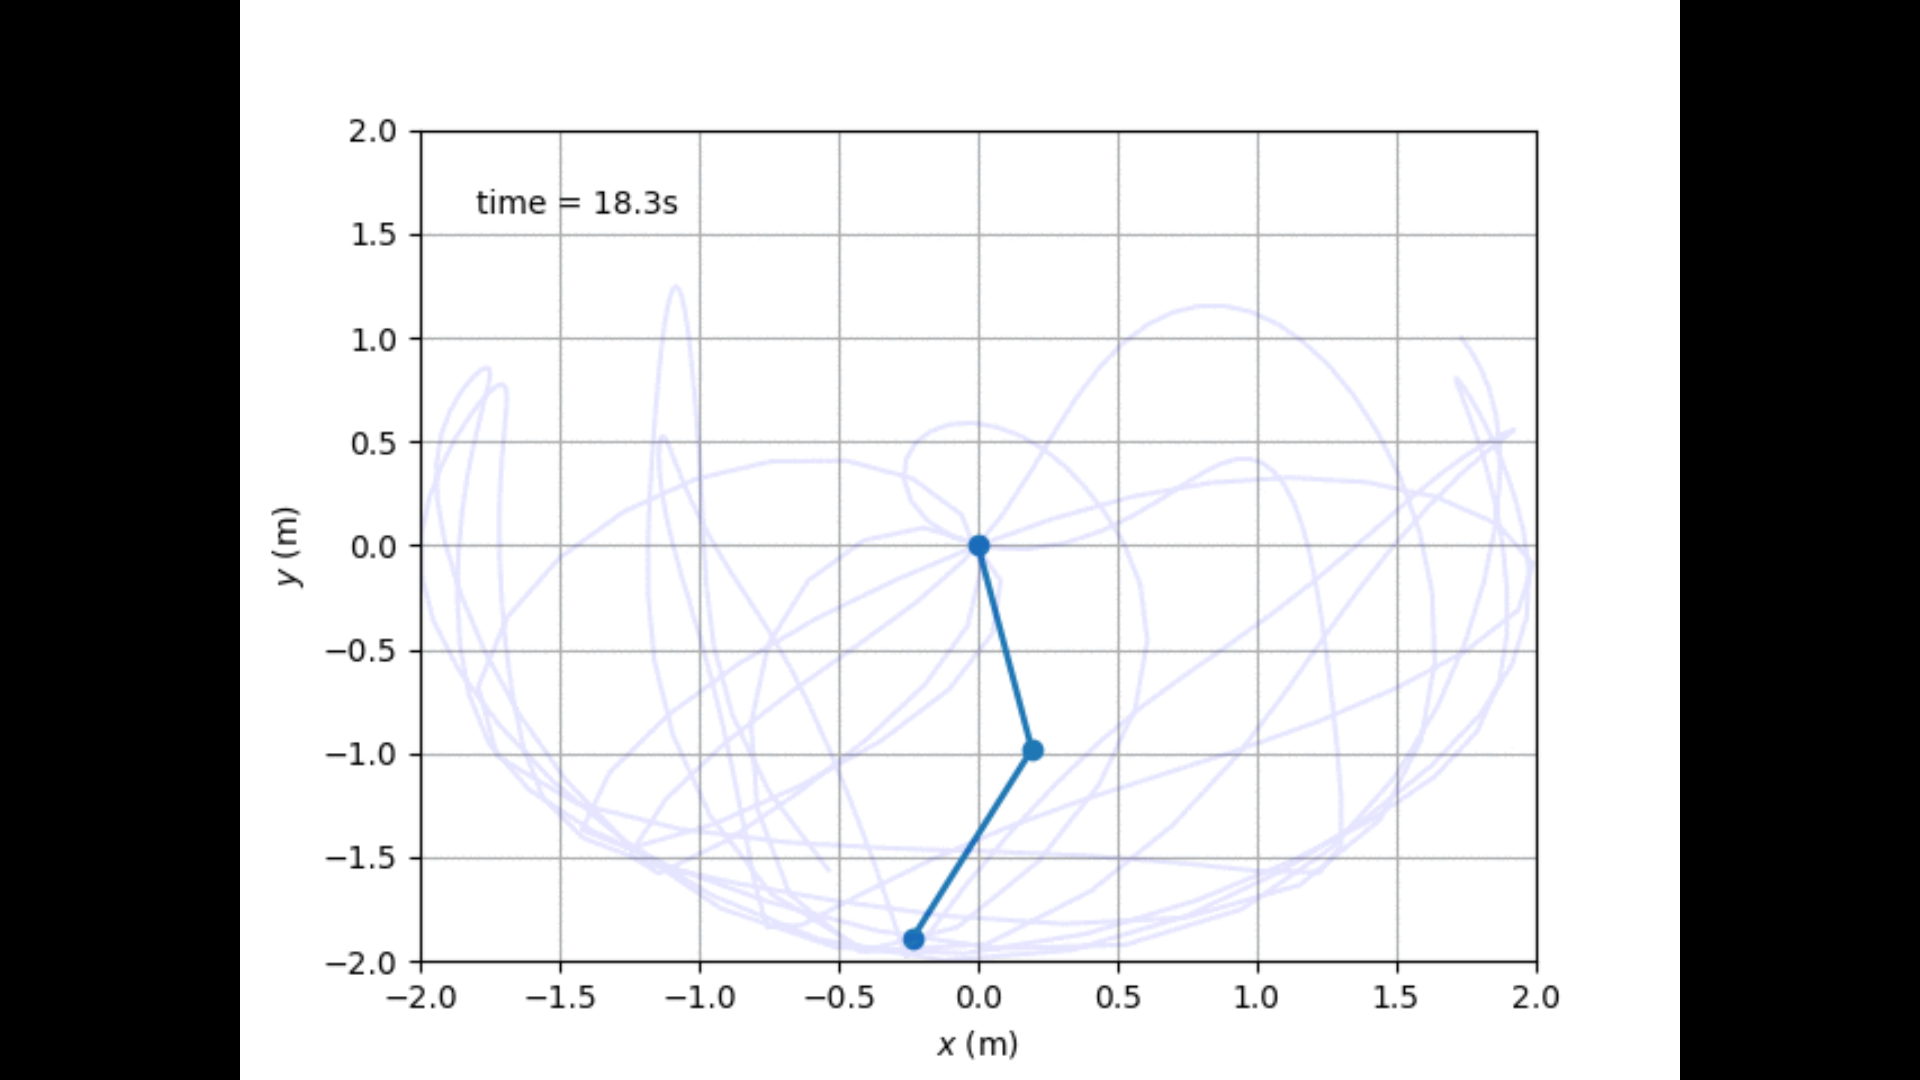
\includegraphics[width = \linewidth]{DP.png}
			\end{columns}
		\end{itemize}
		\bigskip
	\end{frame}
	
	\begin{frame}{Demonstrations}
		\begin{itemize}
			\begin{columns}[t, onlytextwidth]
				\column{.45\textwidth}
					\item\textbf{astrohut} (\url{https://jsbarbosa.github.io/astrohut/})
					
					astrohut is a NBody gravity simulator that aims to help students understand many body systems, as well as motivating the use of computational tools to solve physical problems. Written in Python, with the core functions in C.
					
					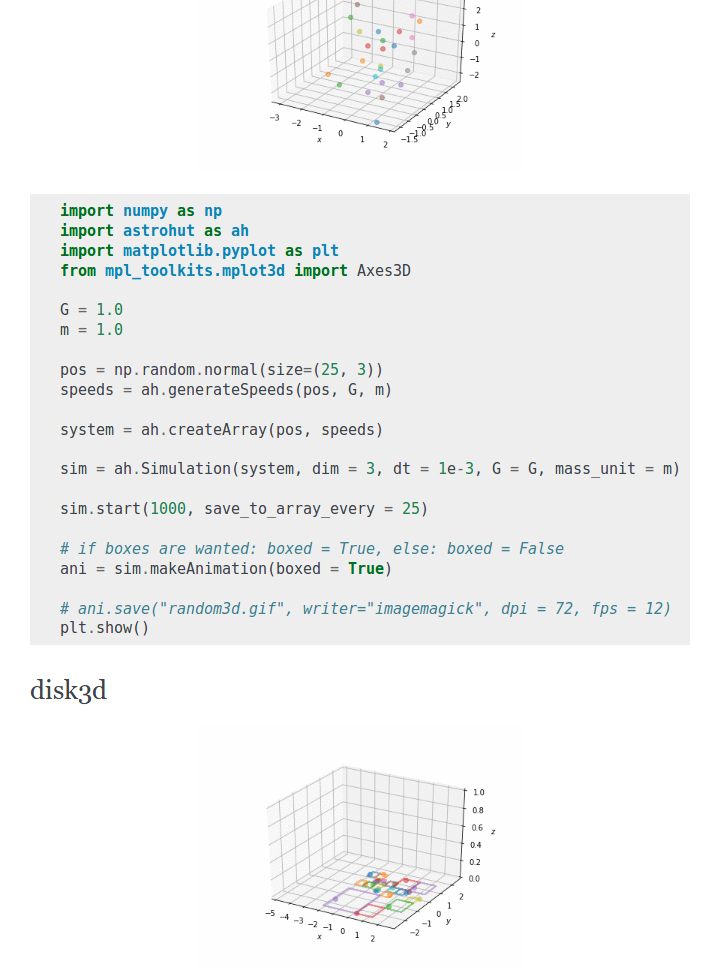
\includegraphics[width=\linewidth]{astroHut.png}
				
				\column{.45\textwidth}
					\item\textbf{rippleTank} (\url{https://jsbarbosa.github.io/rippleTank/})
					
					rippleTank is a simulator that aims to help students understand how waves behave on a ripple tank, as well as motivating the use of computational tools to solve physical problems. Fully written with Python.
					
					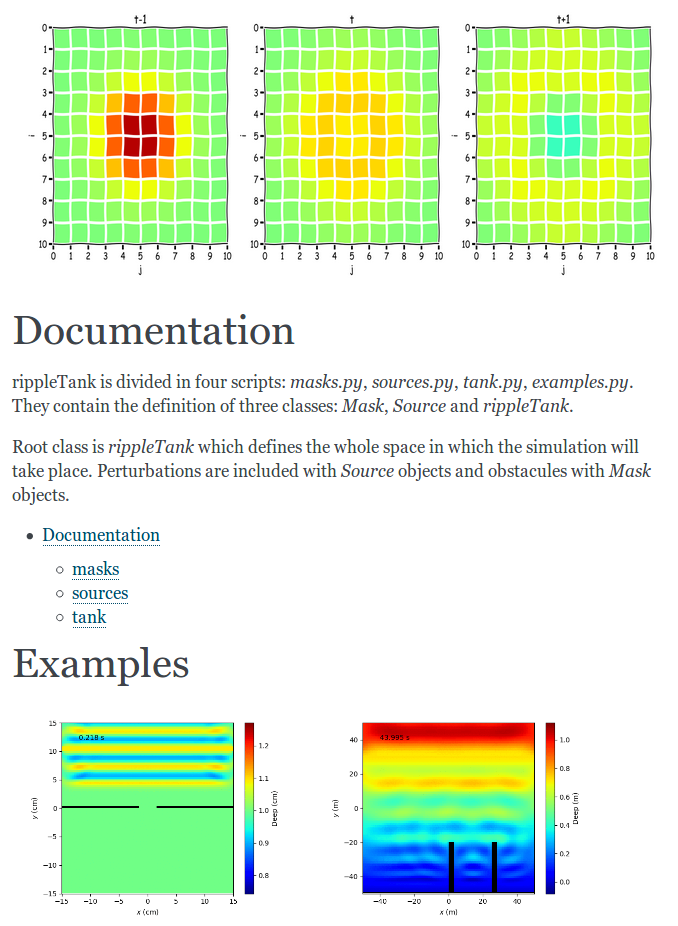
\includegraphics[width=\linewidth]{rippleTank.png}
			\end{columns}
		\end{itemize}
	\end{frame}
	
\end{document}
